%% =============================================================================
%% Data in Brief — Data Descriptor manuscript
%% Main document controller (do not place body text here)
%% Compatible with Overleaf (TeX Live) and local latexmk / pdflatex + bibtex
%% =============================================================================
\documentclass[preprint,12pt]{elsarticle}

%% --- Encoding / fonts --------------------------------------------------------
\usepackage[utf8]{inputenc}   % Safe for older engines; harmless with modern TeX
\usepackage[T1]{fontenc}
\usepackage{lmodern}

%% --- Mathematics / symbols ---------------------------------------------------
\usepackage{amsmath,amssymb}

%% --- Graphics ----------------------------------------------------------------
\usepackage{graphicx}
\graphicspath{{figures/}}
\usepackage[table]{xcolor}    % load before forest to avoid option clash
\usepackage[edges]{forest}    % Figure 1 dataset-structure tree
\usepackage{adjustbox}        % fit Fig. 1 within text width and page height
\definecolor{tablealt}{RGB}{245,247,250}
\definecolor{headergray}{RGB}{55,65,81}

%% --- Tables ------------------------------------------------------------------
\usepackage{booktabs}         % Clean horizontal rules only
\usepackage{tabularx}
\usepackage{multirow}
\usepackage{array}
\usepackage{longtable}

%% --- Captions / floats -------------------------------------------------------
\usepackage{caption}
\usepackage{subcaption}
\usepackage{float}

%% --- Lists -------------------------------------------------------------------
\usepackage{enumitem}

%% --- URLs / hyperlinks -------------------------------------------------------
\usepackage{url}
\usepackage[hidelinks]{hyperref}  % hidelinks: cleaner preprint look

%% --- Bibliography (Elsevier numeric) -----------------------------------------
%% Style applied at \bibliographystyle below; BibTeX keys in references.bib

%% --- Misc --------------------------------------------------------------------
\usepackage{xspace}

%% Optional: uncomment if you need landscape supplementary tables
% \usepackage{pdflscape}

%% -----------------------------------------------------------------------------
\begin{document}

\begin{frontmatter}

\title{NeuroPipeline DICOM Converter: DICOM to BIDS in one workflow}

%% Author block — replace placeholders; add \fnref / \corref as needed
\author[author1]{[TODO: Author Name]}
\author[author2]{[TODO: Author Name]}
%% \author[author3]{[TODO: Author Name]\corref{cor1}}
%% \cortext[cor1]{Corresponding author. Email: [TODO: email@institution.edu]}

\address[author1]{[TODO: Affiliation 1]}
\address[author2]{[TODO: Affiliation 2]}

\begin{abstract}
% Maximum 250 words.
% Self-contained: (1) purpose, (2) population/dataset or tool scope, (3) acquisition,
% (4) processing, (5) main characteristics, (6) availability/usefulness.

% Write the abstract below this line.

\mbox{}

\end{abstract}

\begin{keyword}
[TODO: Keyword 1] \sep
[TODO: Keyword 2] \sep
[TODO: Keyword 3] \sep
[TODO: Keyword 4]
%% Maximum 7 keywords. Remove unused placeholders before submission.
\end{keyword}

\end{frontmatter}

%% --- Specifications table (unnumbered front matter) --------------------------
%% Specifications Table (Data in Brief front matter)
%% Filled only from documented release metadata under scratch (release_dataset/,
%% metadata/participant_mapping.csv). Unverified fields remain marked TODO.
\begin{table}[H]
\centering
\caption{Specifications Table.}
\label{tab:specifications}
\begin{tabular}{@{}p{0.32\linewidth}p{0.62\linewidth}@{}}
\toprule
\textbf{Subject area} & Neuroscience \\
\midrule
\textbf{Specific subject area} &
Multimodal human MRI (structural, functional, diffusion, and field-map imaging)
with four study cohorts labelled in metadata as Control ($n=56$), Glaucoma ($n=19$),
DataON ($n=7$), and DataTON ($n=2$) (84 participants total). \\
\midrule
\textbf{Type of data} &
Raw MRI images (NIfTI); BIDS metadata (JSON, TSV); task event files (where available);
physiological recordings (where conversion gates were met); optional derivatives
(defaced anatomicals; partial preprocessed DWI). \\
\midrule
\textbf{How the data were acquired} &
Siemens Prisma, 3\,T MRI. Longitudinal design with up to two sessions
(\texttt{ses-01}, \texttt{ses-02}). Functional paradigms present in the release include
\texttt{task-rest}, \texttt{task-movie}, \texttt{task-fmri} (visual grating/checkerboard),
and \texttt{task-control}. Conversion to BIDS with dcm2niix / \texttt{neuro\_pipeline}. \\
\midrule
\textbf{Data format} &
BIDS (BIDSVersion 1.9.0); NIfTI (\texttt{.nii.gz}); JSON sidecars; TSV;
physiology \texttt{.tsv.gz} + JSON (where present). \\
\midrule
\textbf{Data source location} &
{[TODO: Institution / city / country --- not stated in the current public release metadata
(administrative institution fields were scrubbed from BIDS sidecars).]} \\
\midrule
\textbf{Data accessibility} &
Repository: FITBIR (accession / URL {[TODO: insert after deposit]}).
Access: restricted under FITBIR data-access agreement (see dataset \texttt{LICENSE}; not CC0). \\
\midrule
\textbf{Related research article} &
{[TODO: Insert related research article citation, or state N/A if none.]} \\
\bottomrule
\end{tabular}
\end{table}

%% Source notes (not printed):
%% - Cohort counts: metadata/participant_mapping.csv (matches 84 sub-* in release_dataset/).
%% - participants.tsv rebuilt 2026-08-16 (was incomplete at 51/84).
%% - Scanner / modalities / tasks / BIDS version: release_dataset/README.md
%% - Access: FITBIR contractual (CC0 withdrawn 2026-08-16)


%% --- Main manuscript sections ------------------------------------------------
\section{Background and Motivation}

\subsection{Background}

% Write here.


\subsection{Motivation}

% Write here.


\section{Data Description}
\label{sec:data_description}

This data release comprises multimodal magnetic resonance imaging (MRI) from a longitudinal visual-system study, organised according to the Brain Imaging Data Structure (BIDS) version~1.9.0 (\texttt{DatasetType}: \texttt{raw}). The packaged tree contains \textbf{84} participants (\texttt{sub-001}--\texttt{sub-084}) and \textbf{135} imaging sessions (\texttt{ses-01}: 83; \texttt{ses-02}: 52). Fifty-one participants have both sessions, 32 have \texttt{ses-01} only, and one participant (\texttt{sub-043}) has \texttt{ses-02} only; unavailable visits are omitted rather than represented by empty folders. Cohort labels in \texttt{participants.tsv} are Control ($n=56$), Glaucoma ($n=19$), DataON ($n=7$; optic neuritis), and DataTON ($n=2$; traumatic optic neuropathy); sex is recorded as Female ($n=46$) and Male ($n=38$). Demographic counts by cohort and session are summarised in Table~\ref{tab:demographics}. Released imaging modalities include anatomical MRI, blood-oxygen-level-dependent (BOLD) functional MRI, spin-echo field maps, and diffusion-weighted MRI, together with task event tables, physiological recordings, and selected derivatives. The overall organisation of the released dataset is illustrated in Fig.~\ref{fig:dataset_overview}.

%% Participant demographics by cohort and session (age omitted).
%% Layout matches reports/participant_summary/Participant_Demographics_by_Session_no_age.png
%% Values match reports/participant_summary/Participant_Demographics_by_Session_no_age.*
\begin{table}[htbp]
\centering
\caption{Participant demographic characteristics by cohort and imaging session (age omitted). Each cohort has ses-01 and ses-02 columns. Values are $n$ or $n$ (\%) as indicated.}
\label{tab:demographics}
\footnotesize
\setlength{\tabcolsep}{4pt}
\renewcommand{\arraystretch}{1.28}
%% tabular (not tabularx) inside resizebox: table keeps the figure's
%% 11-column layout and single-line cells, then scales to \textwidth.
\noindent\resizebox{\textwidth}{!}{%
\begin{tabular}{@{}l*{10}{c}@{}}
\toprule
\textcolor{headergray}{\textbf{Characteristic}} &
\multicolumn{2}{c}{\textcolor{headergray}{\textbf{Control}}} &
\multicolumn{2}{c}{\textcolor{headergray}{\textbf{\shortstack[c]{Optic neuritis\\(ON)}}}} &
\multicolumn{2}{c}{\textcolor{headergray}{\textbf{\shortstack[c]{Traumatic optic\\neuropathy\\(TON)}}}} &
\multicolumn{2}{c}{\textcolor{headergray}{\textbf{Glaucoma}}} &
\multicolumn{2}{c@{}}{\textcolor{headergray}{\textbf{Total}}} \\
\cmidrule(lr){2-3} \cmidrule(lr){4-5} \cmidrule(lr){6-7} \cmidrule(lr){8-9} \cmidrule(l){10-11}
 & \textcolor{headergray}{\textbf{ses-01}} & \textcolor{headergray}{\textbf{ses-02}}
 & \textcolor{headergray}{\textbf{ses-01}} & \textcolor{headergray}{\textbf{ses-02}}
 & \textcolor{headergray}{\textbf{ses-01}} & \textcolor{headergray}{\textbf{ses-02}}
 & \textcolor{headergray}{\textbf{ses-01}} & \textcolor{headergray}{\textbf{ses-02}}
 & \textcolor{headergray}{\textbf{ses-01}} & \textcolor{headergray}{\textbf{ses-02}} \\
\midrule
Participants, $n$
  & 55 & 41
  & 7 & 1
  & 2 & 1
  & 19 & 9
  & 83 & 52 \\
\rowcolor{tablealt}
Female, $n$ (\%)
  & 35 (63.6\%) & 25 (61.0\%)
  & 6 (85.7\%) & 1 (100.0\%)
  & 0 (0.0\%) & 0 (0.0\%)
  & 5 (26.3\%) & 3 (33.3\%)
  & 46 (55.4\%) & 29 (55.8\%) \\
Male, $n$ (\%)
  & 20 (36.4\%) & 16 (39.0\%)
  & 1 (14.3\%) & 0 (0.0\%)
  & 2 (100.0\%) & 1 (100.0\%)
  & 14 (73.7\%) & 6 (66.7\%)
  & 37 (44.6\%) & 23 (44.2\%) \\
\bottomrule
\end{tabular}%
}
\end{table}


\begin{figure}[htbp]
    \centering
    \begin{adjustbox}{max width=\linewidth, max height=0.72\textheight, center}
        \input{figures/fig1_dataset_structure}%
    \end{adjustbox}
    \caption{Overview of the structure of the released multimodal MRI dataset. The dataset is organised according to the Brain Imaging Data Structure (BIDS), with anatomical, functional, diffusion, and field-map data organised within participant and session directories. Task events, physiological recordings, quality-control outputs, processing derivatives, analysis code, and supporting documentation are also provided.}
    \label{fig:dataset_overview}
\end{figure}

At the dataset root, \texttt{dataset\_description.json} records the dataset name, BIDS version, raw dataset type, licence statement, and conversion provenance (\texttt{GeneratedBy}: \texttt{neuro\_pipeline} version~2.1.0). Participant-level metadata are limited to \texttt{participant\_id}, \texttt{cohort}, and \texttt{sex} in \texttt{participants.tsv}, with column definitions in \texttt{participants.json}. Additional root files include \texttt{README.md}, \texttt{CHANGES}, and task metadata sidecars \texttt{task-movie.json}, \texttt{task-movie\_events.json}, and \texttt{task-fmri\_events.json}. A \texttt{code/} directory provides stimulus-related resources used to interpret functional events (including \texttt{presentStimParams.m}, \texttt{task-fmri\_condition\_dictionary.tsv}, \texttt{task-fmri\_condition\_dictionary.json}, and \texttt{code/task-movie/}). Supporting documentation under \texttt{docs/} covers inventory, events, physiology, de-identification, BIDS validation, and quality-control summaries. The file \texttt{.bidsignore} excludes \texttt{*\_TB1TFL*} and \texttt{*\_localizer*} series from BIDS validation while leaving those files present in the tree.

Each packaged session follows the layout \texttt{sub-<id>/ses-<id>/}, with modality folders \texttt{anat/}, \texttt{func/}, \texttt{dwi/}, and \texttt{fmap/} when the corresponding data were collected, and a session-level \texttt{sub-<id>\_ses-<id>\_scans.tsv} listing imaging files in that session (\texttt{acq\_time} is recorded as \texttt{n/a}). Imaging volumes are distributed as gzip-compressed NIfTI (\texttt{*.nii.gz}) with JSON sidecars. Anatomical data under \texttt{anat/} include T1-weighted volumes labelled \texttt{*\_T1w.nii.gz}. Sidecar \texttt{ProtocolName}/\texttt{SeriesDescription} distinguish standard MPRAGE series (\texttt{T1w\_MPR}; 264 volumes in the release) from white-matter-nulled MPRAGE (\texttt{WMn\_MPRAGE\_sagittal}; 118 volumes). Five T1w volumes were withdrawn from the packaged tree after visual QC as unusable (\texttt{docs/quality\_control/excluded\_t1w.md}). Three-dimensional FLAIR volumes (\texttt{*\_FLAIR.nii.gz}; 137 files) are also released. Turbo-flash B1-mapping series (\texttt{*\_TB1TFL.nii.gz}; 272 files) and localizer images are present under \texttt{anat/} but are listed in \texttt{.bidsignore}. Released T1w and FLAIR anatomicals in the BIDS \texttt{anat/} hierarchy are the defaced volumes used for sharing; a separate \texttt{derivatives/defacing/} tree is not duplicated inside this package.

Functional data are stored under \texttt{func/} as magnitude BOLD series (\texttt{*\_bold.nii.gz}) for four task labels: \texttt{task-rest}, \texttt{task-movie}, \texttt{task-fmri}, and \texttt{task-control}. Coverage is incomplete across sessions: the release contains 135 magnitude \texttt{task-rest} runs (132 sessions; typically one run per session), 536 \texttt{task-movie} runs (134 sessions; most often four runs), 553 \texttt{task-fmri} runs (134 sessions; most often four runs), and 401 \texttt{task-control} runs (135 sessions; most often three runs). Representative volume counts in archived magnitude series are 320 (\texttt{task-rest}), 210 (\texttt{task-movie}), 226 (\texttt{task-fmri}), and 20 (\texttt{task-control}); individual runs may differ. Matching single-band reference images (\texttt{*\_sbref.nii.gz}) and phase images (\texttt{part-phase}) are included for many functional acquisitions. Event tables (\texttt{*\_events.tsv}) accompany all 536 magnitude \texttt{task-movie} runs and 514 of the 553 magnitude \texttt{task-fmri} runs; \texttt{task-rest} and \texttt{task-control} have no event files by design. Movie events include \texttt{onset}, \texttt{duration}, \texttt{trial\_type}, \texttt{stim\_file}, \texttt{eye}, \texttt{movie\_label}, and \texttt{matlab\_run\_id}. Task-fMRI events provide block onsets and \texttt{trial\_type} labels (\texttt{baseline} or \texttt{stim-01}--\texttt{stim-12}), with condition definitions in the root and \texttt{code/} dictionaries. Copyrighted movie video files are not redistributed; clip identity is recorded in the event tables and \texttt{code/task-movie/}. Spin-echo EPI field maps under \texttt{fmap/} use opposing phase-encode entities \texttt{dir-AP} and \texttt{dir-PA} (\texttt{*\_epi.nii.gz}; 268 anterior--posterior and 267 posterior--anterior magnitude series in the release, present in all 135 sessions) and are intended for susceptibility distortion correction of EPI data. Field-map sidecars include phase-encoding direction and, where available, \texttt{IntendedFor} references to associated functional or diffusion series.

Diffusion MRI under \texttt{dwi/} is released as \texttt{*\_dwi.nii.gz} with matching JSON sidecars and FSL-style \texttt{*.bval}/\texttt{*.bvec} gradient tables (911 magnitude diffusion series across 131 sessions). Protocol families in the sidecars include gSlider SMS acquisitions (\texttt{gsld\_76dir\_b2000\_1mmiso\_AP}, multi-shell $b=0/1000/2000$~s/mm$^2$; and short posterior--anterior $b=0$ series such as \texttt{gsld\_75TE\_PA\_3b0}) and RESOLVE trace acquisitions (\texttt{resolve\_3scan\_trace\_tra\_p3\_160\_1.4iso\_AP} and \texttt{resolve\_3scan\_trace\_tra\_p3\_160\_1.4iso\_PA}, including TRACEW series; $b=0/1000$~s/mm$^2$ in representative tables). Phase-encoding direction is recorded in the JSON sidecars and varies across runs.

Physiological recordings, when conversion succeeded, are stored alongside the corresponding functional runs as BIDS physiology files \texttt{*\_recording-<channel>\_physio.tsv.gz} with JSON sidecars. Channels present in the release are \texttt{pulse} (1127 files), \texttt{respiratory} (1258), and \texttt{trigger} (1223), totalling 3608 physiology time-series files spanning 77 participants and 116 sessions; absence of physiology for a given run does not by itself indicate invalid BOLD data. Derivatives included under \texttt{derivatives/} are (i) \texttt{mriqc/}, containing native MRIQC image-quality metric JSON for all 84 participants (HTML reports are not packaged), and (ii) \texttt{tractoflow\_normalize\_dwi/}, containing TractoFlow \texttt{Normalize\_DWI} outputs for 66 participants as \texttt{sub-<id>/ses-01/dwi/sub-<id>\_ses-01\_space-dwi\_desc-normalize\_dwi.\{nii.gz,json,bval,bvec\}}. Visual diffusion QC materials associated with that derivative are provided under \texttt{docs/quality\_control/dwi/}.

\section{MRI Data Acquisition}
\label{sec:mri_acquisition}

MRI sessions followed a multimodal acquisition framework that was broadly consistent
across complete visits, although the exact set, number, and order of acquisitions varied
according to the study protocol and participant group. Complete examination sessions
typically lasted approximately 115--135\,min. The description below summarizes the overall
organization of the examination, while detailed acquisition parameters are provided
separately in Table~\ref{tab:mri_acq_parameters}.

%% MRI acquisition parameters (representative values from released BIDS sidecars).
%% Companion to the session-organisation paragraph in sec:mri_acquisition.
%% Diffusion rows align with docs/diffusion/diffusion_acquisition_parameters.tsv.
\begin{table}[htbp]
\centering
\caption{MRI acquisition parameters for the principal sequences in the release.
Values are representative parameters taken from packaged BIDS JSON sidecars
(Siemens Prisma~3\,T, 64-channel head/neck coil). Exact run counts and console
order varied across sessions; \texttt{run} indices are assigned at conversion.
Diffusion rows distinguish raw gSlider slab geometry from the reconstructed
1\,mm \texttt{Normalize\_DWI} derivative. Localizer series were acquired for
prescription but are not packaged in the release.}
\label{tab:mri_acq_parameters}
\footnotesize
\setlength{\tabcolsep}{3.5pt}
\renewcommand{\arraystretch}{1.15}
\begin{adjustbox}{max width=\textwidth,center}
\begin{tabular}{@{}>{\raggedright\arraybackslash}p{2.6cm}
                >{\raggedright\arraybackslash}p{2.4cm}
                >{\raggedright\arraybackslash}p{2.1cm}
                c
                >{\raggedright\arraybackslash}p{2.0cm}
                >{\raggedright\arraybackslash}p{3.6cm}@{}}
\toprule
\textcolor{headergray}{\textbf{Sequence}} &
\textcolor{headergray}{\textbf{ProtocolName}} &
\textcolor{headergray}{\textbf{Voxel size (mm)}} &
\textcolor{headergray}{\textbf{TR / TE (/ TI)}} &
\textcolor{headergray}{\textbf{FA / accel.}} &
\textcolor{headergray}{\textbf{Notes}} \\
\midrule
\multicolumn{6}{@{}l}{\textit{Anatomical}} \\
\midrule
T1w MPRAGE & \texttt{T1w\_MPR} & $0.8$ iso & $2500$ / $2.22$ / $1000$\,ms & $8^\circ$; iPAT\,2 & Typically two runs/session; \texttt{run-02} usually reconstructed with Siemens \texttt{NORM} \\
\rowcolor{tablealt}
WMn MPRAGE & \texttt{WMn\_MPRAGE\_sagittal} & $1.0$ iso & $4000$ / $3.82$ / $500$\,ms & $7^\circ$; iPAT\,2 & White-matter-nulled; usually \texttt{run-03\_T1w} \\
3D FLAIR & \texttt{Sag Flair 3D-0.8} & $0.8$ iso & $6000$ / $357$ / $2200$\,ms & $120^\circ$; iPAT\,2 & One run/session in most visits \\
\rowcolor{tablealt}
B1 map & \texttt{tfl\_b1map\_1mmiso} & $\sim 3.4\times3.4\times10$ & $4000$ / $1.83$\,ms & $8^\circ$ & 15 slices (thickness 8\,mm, spacing 10\,mm); gSlider B1 calibration (\texttt{TB1TFL}) \\
\midrule
\multicolumn{6}{@{}l}{\textit{Functional BOLD (MB8 EPI; tasks share geometry)}} \\
\midrule
BOLD (all tasks) & \texttt{REST*}/\texttt{Movie*}/\texttt{fMRI*}/\texttt{Control*} & $2.0$ iso & $937$ / $37$\,ms & $52^\circ$; MB\,8 & Matrix $104\times104\times88$; BW $\sim$2290\,Hz/Px; PE mainly AP (some control runs PA). Representative lengths: rest $\sim$320, movie $\sim$210, fmri $\sim$226, control $\sim$20 vols \\
\midrule
\multicolumn{6}{@{}l}{\textit{Field maps}} \\
\midrule
Spin-echo EPI fmap & \texttt{SpinEchoFieldMap\_AP/PA} & $2.0$ iso & $9710$ / $66$\,ms & $90^\circ$ & Opposing PE (\texttt{dir-AP}/\texttt{dir-PA}); matched to BOLD FOV/matrix for distortion correction \\
\midrule
\multicolumn{6}{@{}l}{\textit{Diffusion}} \\
\midrule
gSlider-SMS AP & \texttt{gsld\_76dir\_b2000\_1mmiso\_AP} & Raw $1\times1\times5$ (30 slabs); recon.\ $1$ iso & $3500$ / $75$\,ms & $90^\circ$; MB\,2; iPAT\,3; PF\,6/8 & Multi-shell $b=0/1000/2000$\,s/mm$^2$. Raw series retain RF encodings (modal 385 time points). Analysis-ready: $4\,b0+37+36=77$ vols in \texttt{Normalize\_DWI} \\
\rowcolor{tablealt}
gSlider PA $b=0$ & \texttt{gsld\_75TE\_PA\_3b0} & Raw $1\times1\times5$ & $3500$ / $75$\,ms & $90^\circ$; MB\,2; iPAT\,3; PF\,6/8 & Reverse-PE $b=0$ references (modal 5 vols); for topup \\
RESOLVE trace AP & \texttt{resolve\_\ldots{}1.4iso\_AP} & $\sim 1.38\times1.38\times1.82$ & $4140$ / $51$\,ms & $180^\circ$; iPAT\,3 & Clinical RESOLVE; $b=0/1000$\,s/mm$^2$ (modal 15 vols); TRACEW products also released \\
\rowcolor{tablealt}
RESOLVE PA & \texttt{resolve\_\ldots{}1.4iso\_PA} & $\sim 1.38\times1.38\times1.82$ & $\sim 24.8$\,s / $51$\,ms & $180^\circ$; iPAT\,3 & Primarily reverse-PE $b=0$ (modal 3 vols) \\
\bottomrule
\end{tabular}
\end{adjustbox}
\end{table}


\subsection{MRI Scanner}

% Write here.


\subsection{Anatomical MRI}

% Write here. Cite Table~\ref{tab:mri_acquisition} for laboratory series$\rightarrow$BIDS filename mapping.

%% MRI acquisition protocol: laboratory SeriesDescription → BIDS
%% Layout matches reports/pi_pipeline_briefing/figures/Table_MRI_acquisition_protocol_lab_to_bids.png
\begin{table}[htbp]
\centering
\caption{MRI acquisition protocol: laboratory SeriesDescription mapped to BIDS datatype and general filename pattern (single session, console order). Run index $<$N$>$ is assigned at conversion and may differ from acquisition order. Full form: \texttt{sub-<ID>\_ses-<01|02>\_<entities>\_<suffix>.nii.gz}.}
\label{tab:mri_acquisition}
\footnotesize
\setlength{\tabcolsep}{4pt}
\renewcommand{\arraystretch}{1.22}
%% Shrink only if the 11pt/wide-figure layout exceeds manuscript \textwidth.
\begin{adjustbox}{max width=\textwidth,center}
\begin{tabular}{@{}c l c l@{}}
\toprule
\textcolor{headergray}{\textbf{\#}} &
\textcolor{headergray}{\textbf{Lab series name}} &
\textcolor{headergray}{\textbf{BIDS datatype}} &
\textcolor{headergray}{\textbf{General BIDS name}} \\
\midrule
1 & \texttt{Localizer} & \texttt{anat} & \texttt{run-\textless{}N\textgreater{}\_localizer} \\
\rowcolor{tablealt}
2 & \texttt{fMRI1\_AP} & \texttt{func} & \texttt{task-fmri\_run-\textless{}N\textgreater{}\_bold} \\
3 & \texttt{fMRI2\_AP} & \texttt{func} & \texttt{task-fmri\_run-\textless{}N\textgreater{}\_bold} \\
\rowcolor{tablealt}
4 & \texttt{Control1\_PA} & \texttt{func} & \texttt{task-control\_run-\textless{}N\textgreater{}\_bold} \\
5 & \texttt{fMRI3\_AP} & \texttt{func} & \texttt{task-fmri\_run-\textless{}N\textgreater{}\_bold} \\
\rowcolor{tablealt}
6 & \texttt{fMRI4\_AP} & \texttt{func} & \texttt{task-fmri\_run-\textless{}N\textgreater{}\_bold} \\
7 & \texttt{Movie1\_AP} & \texttt{func} & \texttt{task-movie\_run-\textless{}N\textgreater{}\_bold} \\
\rowcolor{tablealt}
8 & \texttt{Movie2\_AP} & \texttt{func} & \texttt{task-movie\_run-\textless{}N\textgreater{}\_bold} \\
9 & \texttt{SpinEchoFieldMap\_AP} & \texttt{fmap} & \texttt{dir-AP\_run-\textless{}N\textgreater{}\_epi} \\
\rowcolor{tablealt}
10 & \texttt{SpinEchoFieldMap\_PA} & \texttt{fmap} & \texttt{dir-PA\_run-\textless{}N\textgreater{}\_epi} \\
11 & \texttt{Movie3\_AP} & \texttt{func} & \texttt{task-movie\_run-\textless{}N\textgreater{}\_bold} \\
\rowcolor{tablealt}
12 & \texttt{Movie4\_AP} & \texttt{func} & \texttt{task-movie\_run-\textless{}N\textgreater{}\_bold} \\
13 & \texttt{REST1\_AP} & \texttt{func} & \texttt{task-rest\_run-\textless{}N\textgreater{}\_bold} \\
\midrule
\textbf{*} & & & \\
\midrule
\rowcolor{tablealt}
14 & \texttt{Localizer} & \texttt{anat} & \texttt{run-\textless{}N\textgreater{}\_localizer} \\
15 & \texttt{T1w\_MPR} & \texttt{anat} & \texttt{run-\textless{}N\textgreater{}\_T1w} \\
\rowcolor{tablealt}
16 & \texttt{Control2\_AP} & \texttt{func} & \texttt{task-control\_run-\textless{}N\textgreater{}\_bold} \\
17 & \texttt{Control3\_PA} & \texttt{func} & \texttt{task-control\_run-\textless{}N\textgreater{}\_bold} \\
\rowcolor{tablealt}
18 & \texttt{SpinEchoFieldMap\_AP} & \texttt{fmap} & \texttt{dir-AP\_run-\textless{}N\textgreater{}\_epi} \\
19 & \texttt{SpinEchoFieldMap\_PA} & \texttt{fmap} & \texttt{dir-PA\_run-\textless{}N\textgreater{}\_epi} \\
\rowcolor{tablealt}
20 & \texttt{gsld\_76dir\_b2000\_1mmiso\_AP} & \texttt{dwi} & \texttt{run-\textless{}N\textgreater{}\_dwi} \\
21 & \texttt{gsld\_75TE\_PA\_3b0} & \texttt{dwi} & \texttt{run-\textless{}N\textgreater{}\_dwi} \\
\rowcolor{tablealt}
22 & \texttt{tfl\_b1map\_1mmiso} & \texttt{anat} & \texttt{run-\textless{}N\textgreater{}\_TB1TFL} \\
23 & \texttt{resolve\_3scan\_trace\_tra\_p3\_160\_1.4iso\_AP} & \texttt{dwi} & \texttt{run-\textless{}N\textgreater{}\_dwi} \\
\rowcolor{tablealt}
24 & \texttt{resolve\_3scan\_trace\_tra\_p3\_160\_1.4iso\_PA} & \texttt{dwi} & \texttt{run-\textless{}N\textgreater{}\_dwi} \\
25 & \texttt{Sag Flair 3D-0.8} & \texttt{anat} & \texttt{run-\textless{}N\textgreater{}\_FLAIR} \\
\rowcolor{tablealt}
26 & \texttt{WMn\_MPRAGE\_sagittal} & \texttt{anat} & \texttt{run-\textless{}N\textgreater{}\_T1w} \\
\bottomrule
\end{tabular}
\end{adjustbox}

\vspace{4pt}
\begin{flushleft}
\footnotesize
\textbf{*} Anterior part of the head coil added, after which the localizer is repeated.
\end{flushleft}
\end{table}


\subsection{Functional MRI}

% Write here.


\subsection{Field Maps}

% Write here.


\subsection{Diffusion MRI}

\begin{figure}[htbp]
\centering
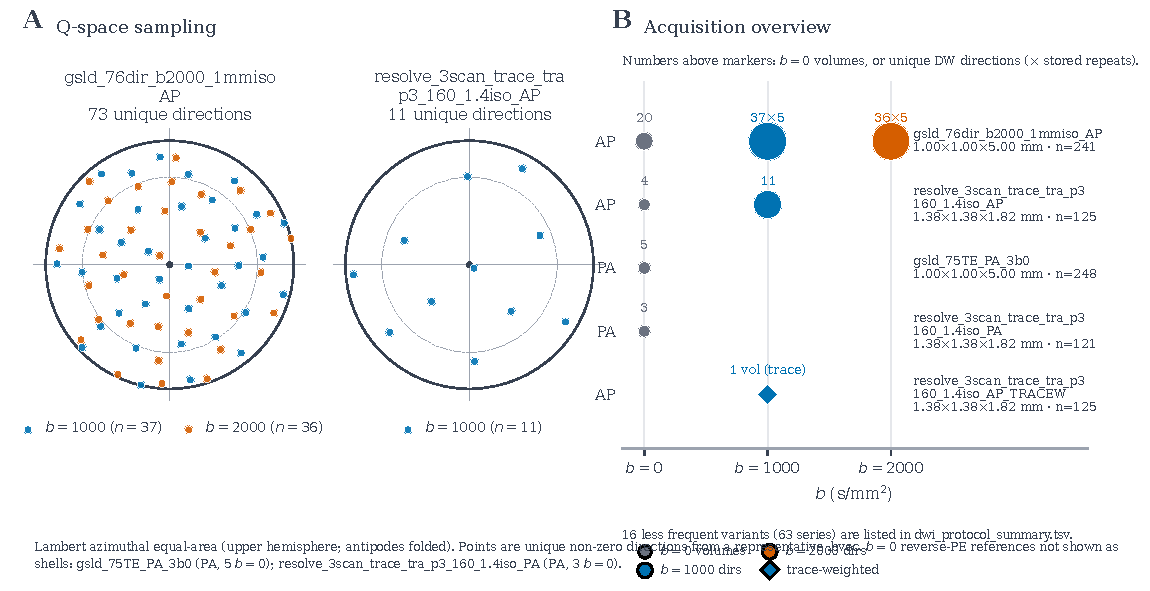
\includegraphics[width=\linewidth]{figures/Figure_DWI_protocols.pdf}
\caption{Diffusion MRI acquisition schemes in the released BIDS dataset. (A)~Angular distribution of unique non-zero diffusion-encoding directions from representative \texttt{.bvec} files, shown as a Lambert azimuthal equal-area projection of the upper hemisphere (antipodal directions folded). \texttt{gsld\_76dir\_b2000\_1mmiso\_AP} [AP: $b=1000$ ($n=37$ unique directions), $b=2000$ ($n=36$ unique directions)]; \texttt{resolve\_3scan\_trace\_tra\_p3\_160\_1.4iso\_AP} [AP: $b=1000$ ($n=11$ unique directions)]. Reverse-phase-encoding $b=0$ series (\texttt{gsld\_75TE\_PA\_3b0} [PA]; \texttt{resolve\_3scan\_trace\_tra\_p3\_160\_1.4iso\_PA} [PA]) are reference images and are not plotted as diffusion shells. (B)~Protocol-level summary of $b$-value shells, unique angular samples per shell, $b=0$ volume counts, voxel size, phase-encoding direction, and number of magnitude series for schemes represented in $\geq$20 series. The figure is derived from 923 released DWI NIfTI files in 131 sessions and shows unique acquisition schemes rather than every individual series. Where a gradient table stores repeated encodings of the same direction, panel~A plots unique directions and panel~B reports the observed repeat factor. 16 less frequent variants (truncated shells, alternate voxel size, missing phase-encoding metadata, or shim/PE differences) are tabulated in \texttt{dwi\_protocol\_summary.tsv}.}
\label{fig:dwi_protocols}
\end{figure}


% Write here. Cite Fig.~\ref{fig:dwi_protocols}.


\subsection{Physiological Recordings}

% Write here.


\section{Experimental Paradigms}
\label{sec:experimental_paradigms}

\subsection{Grating Task}

% Write here.


\subsection{Movie Paradigm}

% Write here.


\subsection{Control Condition}

% Write here.


\subsection{Resting-State Paradigm}

% Write here.


\section{Data Processing}
\label{sec:data_processing}

\begin{figure}[htbp]
    \centering
    \begin{adjustbox}{max width=\linewidth, center}
        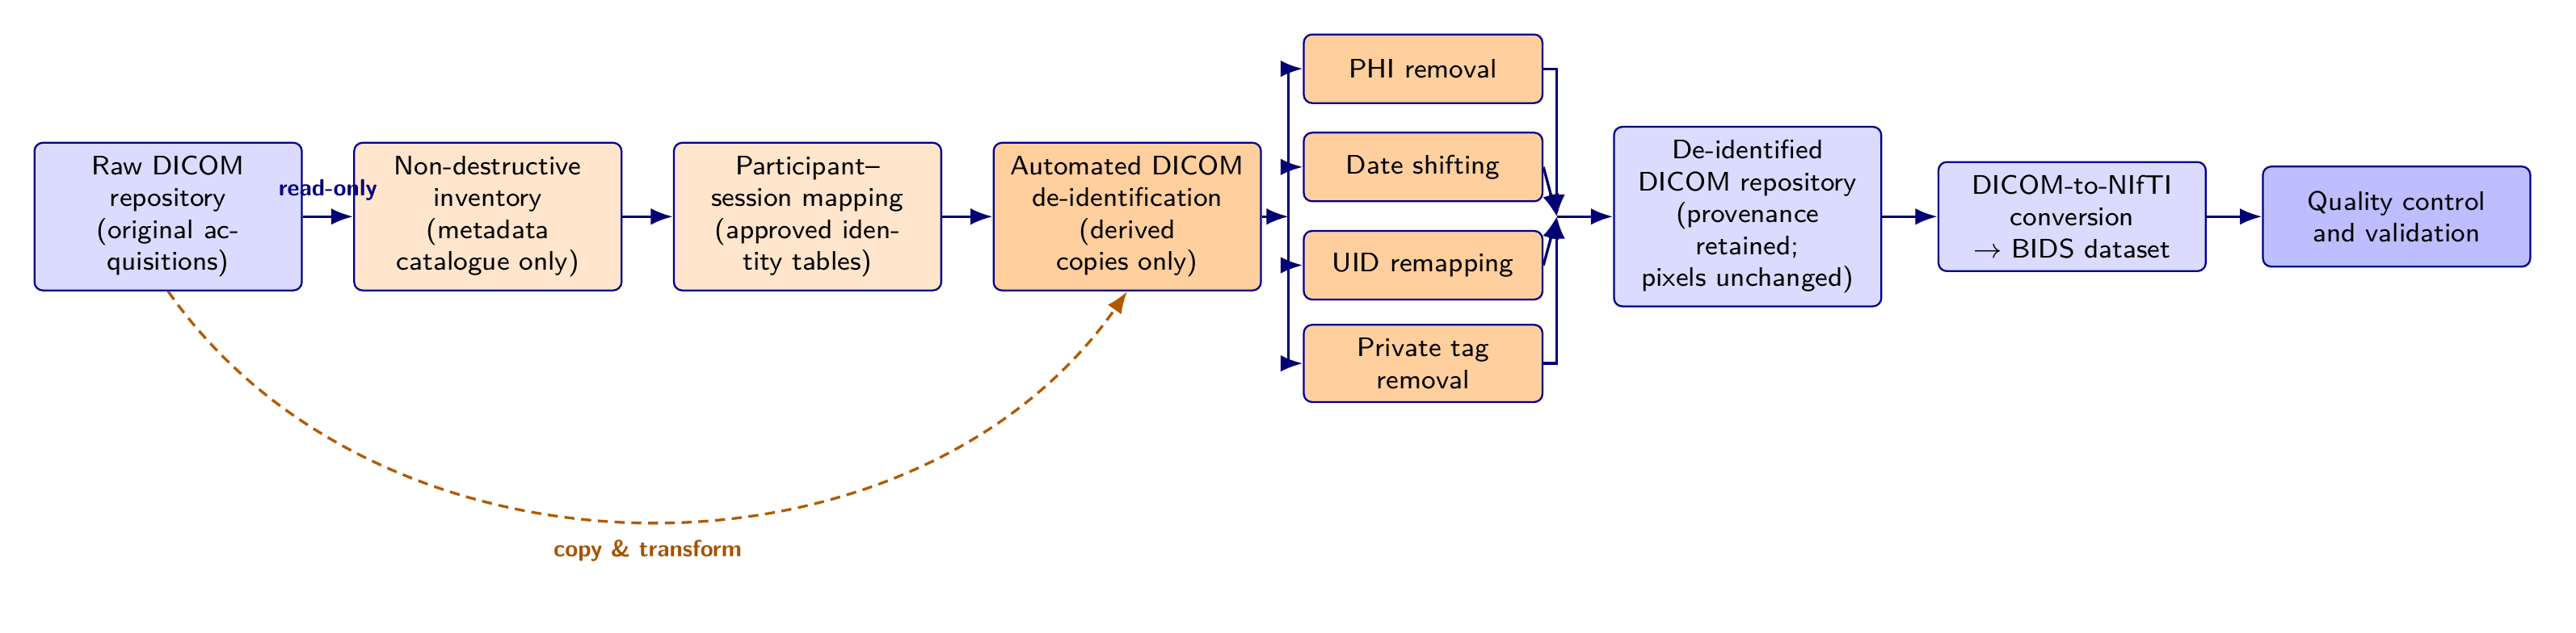
\includegraphics[width=\linewidth]{figures/Figure_2.png}%
    \end{adjustbox}
    \caption{De-identification and release-preparation workflow. Downstream processing uses derived copies; the raw archive is never overwritten.}
    \label{fig:processing_workflow}
\end{figure}

\subsection{DICOM-to-BIDS conversion and dataset construction}
\label{sec:dicom_to_bids}

\subsubsection{DICOM inventory and series identification}

Source DICOM series were inventoried from the original scanner archive without modifying that archive. Each series was assigned pseudonymous BIDS entities---participant label (\texttt{sub-<ID>}), session (\texttt{ses-01} or \texttt{ses-02}), modality folder, and run index---using study mapping tables frozen before conversion. Mapping overrides applied at that stage are documented in \texttt{docs/inventory/MAPPING\_OVERRIDES.md}. Sequence-level coverage and missing families are recorded in \texttt{docs/inventory/}.

\subsubsection{DICOM-to-NIfTI conversion}

De-identified working copies of the DICOM data were converted to gzip-compressed NIfTI with JSON sidecars using \texttt{dcm2niix} (version 1.0.20230411; arguments \texttt{-b y -ba y -z y}). Conversion and BIDS organisation were orchestrated by \texttt{neuro\_pipeline} version 2.1.0, as recorded in \texttt{dataset\_description.json}. After conversion, JSON sidecars were scrubbed of residual personal and institutional identifiers; missing \texttt{TaskName} values were injected from filenames when needed; phase images were renamed to the BIDS \texttt{part-phase} entity; and field-map \texttt{IntendedFor} targets were set where applicable. For Siemens XA30 Enhanced MR sessions in which \texttt{dcm2niix} did not export \texttt{SliceTiming}, values were recovered from DICOM frame timing (\texttt{FrameAcquisitionDateTime} / \texttt{InStackPositionNumber}) when available.

\subsubsection{BIDS organization and naming}

Converted data were organised according to BIDS version 1.9.0 (\texttt{DatasetType}: \texttt{raw}). Imaging files were placed under \texttt{sub-<ID>/ses-<ID>/\{anat,func,dwi,fmap\}/} with standard entities (for example \texttt{task-}, \texttt{run-}, \texttt{dir-AP}/\texttt{dir-PA}, \texttt{part-phase}). Diffusion series include companion \texttt{.bval} and \texttt{.bvec} files. Session-level \texttt{*_scans.tsv} tables list imaging files within each session. Structural compliance of the MRI imaging tree was checked with bids-validator version 1.15.0 (MRI imaging scope; physiology and events documented separately). Remediation preceding the validation snapshot included field-map metadata repairs, filename and entity fixes, XA30 \texttt{SliceTiming} recovery, and inclusion of verified event tables. Remaining validator warnings were reviewed and disclosed rather than suppressed.

\subsection{Diffusion MRI preprocessing}
\label{sec:dwi_preprocessing}

Preprocessed multi-shell diffusion MRI is released under \texttt{derivatives/tractoflow\_normalize\_dwi/} for 66 participants (49 Control and 17 Glaucoma; one session each: \texttt{ses-01}, except \texttt{sub-066}/\texttt{ses-02}). This derivative is the TractoFlow \texttt{Normalize\_DWI} product for the gSlider-SMS acquisitions (\texttt{gsld\_76dir\_b2000\_1mmiso\_AP}), not for the clinical RESOLVE series. Files are named \texttt{sub-<id>\_ses-<id>\_space-dwi\_desc-normalize\_dwi.\{nii.gz,json,bval,bvec\}}. They are analysis-ready derivatives and do not replace the raw BIDS \texttt{dwi/} runs. HCP structural derivatives, fibre-orientation maps, and tractograms are not packaged in this tree.

The raw gSlider volumes retain slab RF encodings (modal geometry $1 \times 1 \times 5$~mm, typically 385 time points, shells $b=0/1000/2000$~s/mm$^2$). Before TractoFlow, gSlider data were reconstructed to 1~mm isotropic diffusion volumes and corrected for $B_1$ inhomogeneity using the turbo-flash $B_1$ maps acquired in the same sessions (\texttt{tfl\_b1map\_1mmiso} / \texttt{TB1TFL}) \cite{liao2020gslider}. Reverse phase-encode $b=0$ gSlider references (\texttt{gsld\_75TE\_PA\_3b0}) were used for susceptibility-distortion correction.

A well-designed pre- and post-processing stream is critical for robust tractography. In the IronTract challenge, replacing candidate preprocessing methods with a top-ranking pipeline improved results \cite{maffei2022irontract}. Diffusion preprocessing therefore used a modified TractoFlow pipeline \cite{theaud2020tractoflow} informed by the IronTract and DiSCo challenges \cite{girard2023disco}. Relative to default TractoFlow, denoising used NORDIC \cite{moeller2021nordic} rather than the standard MP-PCA step, and orientation-distribution-function estimation was updated (those fODF products are not in this release). The stream applied to the volumes packaged here comprised NORDIC denoising, Gibbs-ringing correction \cite{kellner2016gibbs}, and correction for motion, eddy currents, and susceptibility distortions with FSL TOPUP and EDDY \cite{andersson2003topup,andersson2016eddy}, followed by N4 bias-field correction (ANTs), resampling to 1~mm isotropic resolution, and intensity normalization. The released volumes remain in native diffusion space and are not skull-stripped. Each series contains 77 volumes (4 $b=0$, 37 $b=1000$~s/mm$^2$, 36 $b=2000$~s/mm$^2$; 73 unique non-$b=0$ directions). A representative reconstructed matrix is $147 \times 183 \times 145$. TractoFlow also takes a T1-weighted volume; the collaborator QC registered that T1 into diffusion space, but T1/FLAIR anatomy is not duplicated inside \texttt{tractoflow\_normalize\_dwi/}. Visual QC of this derivative is described in Section~\ref{sec:quality_control}.

\subsection{Physiological data processing}
\label{sec:physiology_processing}

Siemens PhysioLog DICOM were converted to BIDS physiology files (\texttt{*_recording-<channel>\_physio.tsv.gz} with matching JSON sidecars) only when release gates were met: usable sampling metadata, a derivable start time relative to the linked BOLD series, and a unique BOLD association. Channels written under this policy are \texttt{pulse}, \texttt{respiratory}, and \texttt{trigger} (ECG was not retained in the packaged tree). Sidecars were restricted to an allowlisted metadata set, including \texttt{SamplingFrequency}, \texttt{StartTime}, \texttt{StartTimeMethod}, and \texttt{StartTimeConfidence}. Failed-gate PhysioLogs and session-wide peripheral PMU logs without unique run linkage were not written into the BIDS tree. Physiology files, when present, are colocated with the corresponding functional run under \texttt{func/}. Absence of physiology for a given run indicates a failed conversion gate or no archived PhysioLog for that acquisition, not an invalid BOLD series. Eye-tracking time series are not included in this release.

\subsection{Event and stimulus metadata processing}
\label{sec:events_processing}

Task event tables were generated from experimental records only when a unique protocol-to-BOLD correspondence could be established. For \texttt{task-fmri}, \texttt{*_events.tsv} files provide \texttt{onset}, \texttt{duration}, and \texttt{trial\_type} (\texttt{baseline} or \texttt{stim-01}--\texttt{stim-12}); onsets were reconstructed from measured scanner trigger recordings combined with stimulus-order metadata, without substituting a default TR or inventing onsets for unmatched runs. Condition definitions are provided in \texttt{code/task-fmri\_condition\_dictionary.tsv} (with JSON sidecar) and dataset-root \texttt{task-fmri\_events.json}; the canonical stimulus script \texttt{code/presentStimParams.m} is released for provenance. For \texttt{task-movie}, design-level events accompany magnitude movie runs and include \texttt{onset}, \texttt{duration}, \texttt{trial\_type}, \texttt{stim\_file}, \texttt{eye}, \texttt{movie\_label}, and \texttt{matlab\_run\_id} (definitions in \texttt{task-movie\_events.json}). Movie timing uses \texttt{onset = 0} under the documented protocol assumption that acquisition and clip playback started together; these events are not millisecond TTL-locked onsets. Copyrighted movie video files are not redistributed. Resting-state and control runs have no event files by design. Event inventories are summarised under \texttt{docs/events/}.

\subsection{De-identification and privacy protection}
\label{sec:deidentification}

DICOM de-identification was applied to mapped working copies before NIfTI conversion; original scanner exports remained an unmodified archive. Header processing followed a custom attribute-confidentiality policy oriented toward the DICOM PS3.15 Basic Application Level Confidentiality Profile (curated tag actions; not claimed as certified full-profile compliance). Direct identifiers were replaced with study codes; institutional, physician, accession, device-serial, and related free-text identifier fields were cleared; private tags were removed except where required for reconstruction metadata; UIDs were deterministically remapped; and calendar dates were shifted by a participant-specific offset while preserving longitudinal intervals. Acquisition parameters required for analysis (including series descriptions) and participant sex were retained by default. Image pixel values were not altered during DICOM header de-identification. After conversion, BIDS JSON sidecars were re-scrubbed and audited for residual forbidden personal or institutional fields. The public \texttt{participants.tsv} is limited to \texttt{participant\_id}, \texttt{cohort}, and \texttt{sex}. Source DICOM is not redistributed. Anatomical facial features on shared T1-weighted and FLAIR volumes were removed with \texttt{pydeface} (version 2.0.0+computecanada) and FSL (version 6.0.7.20); in this package the defaced anatomicals are distributed in the BIDS \texttt{anat/} hierarchy. Identity mapping tables and the per-subject date-shift table are not included. De-identification audits are provided under \texttt{docs/deidentification/}.

\section{Quality Control}
\label{sec:quality_control}

\begin{figure}[htbp]
    \centering
    % \includegraphics[width=\linewidth]{figures/Figure_4.pdf}
    \fbox{\parbox[c][0.28\linewidth][c]{0.92\linewidth}{\centering
    Placeholder for Figure~4 --- Quality control / completeness.\\
    Add \texttt{figures/Figure\_4.pdf} and uncomment \texttt{\textbackslash includegraphics}.}}
    \caption{Overview of MRIQC and diffusion QC coverage and outcomes for the released dataset.}
    \label{fig:quality_control}
\end{figure}

Quality control (QC) for this release comprises two complementary layers: (i)~automated image-quality metrics (IQMs) from MRIQC applied to magnitude anatomical T1-weighted and functional BOLD series in the BIDS tree, and (ii)~visual / protocol QC of the packaged TractoFlow-normalized diffusion derivative using \texttt{scilus/dmriqc\_flow} reports provided by the collaborator share. QC outputs are intended to characterise acquisitions and to prioritise inspection; they were not used as automatic exclusion criteria unless a specific artefact states otherwise. Five T1w volumes were subsequently withdrawn from the packaged tree after visual inspection found them unusable (\texttt{docs/quality\_control/excluded\_t1w.md}). Tabular summaries and report packages are distributed under \texttt{docs/quality\_control/}, with native MRIQC JSON under \texttt{derivatives/mriqc/}.

\subsection{Sequences included in QC}

MRIQC was applied to magnitude \texttt{T1w} volumes under \texttt{anat/} and magnitude BOLD series under \texttt{func/} (\texttt{task-rest}, \texttt{task-movie}, \texttt{task-fmri}, and \texttt{task-control}). The expected set for this layer is defined as every magnitude T1w or BOLD NIfTI present in the release BIDS tree (2007 expected runs across 84 participants and 135 sessions). FLAIR, B1-mapping (\texttt{TB1TFL}), localizers, phase images, spin-echo field maps, and raw BIDS \texttt{dwi/} series were not scored by MRIQC in the packaged campaign.

Diffusion QC covers the TractoFlow \texttt{Normalize\_DWI} derivative in \texttt{derivatives/tractoflow\_normalize\_dwi/} for 66 subjects (one session each: 49 Control and 17 Glaucoma), corresponding to multi-shell acquisitions with $b=0/1000/2000$~s/mm$^2$ and 77 directions. This QC evaluates the normalized DWI and a T1 volume registered into diffusion space; it is not a substitute for QC of all raw BIDS diffusion runs (more subjects have raw \texttt{dwi/} than have the normalized derivative).

\subsection{MRIQC procedures}

MRIQC jobs targeted the \texttt{nipreps/mriqc:24.0.2} container; per-run JSON record \texttt{provenance.version} \texttt{24.1.0.dev0+gd5b13cb5.d20240826} for all successful outputs. Anatomical jobs used modality \texttt{T1w} and functional jobs modality \texttt{bold}. Native IQMs (for example contrast-to-noise and coefficient of joint variation for T1w; mean framewise displacement, temporal SNR, and DVARS-related metrics for BOLD) were written as JSON under \texttt{derivatives/mriqc/} and aggregated into \texttt{docs/quality\_control/mriqc/mriqc\_metrics.csv}. HTML/SVG participant reports are not packaged because MRIQC was run on pre-deface T1w inputs and the HTML mosaics would expose identifiable facial structure; users should rely on the JSON IQMs and publication tables under \texttt{docs/quality\_control/mriqc/}.

In addition to native MRIQC metrics, project-derived exploratory outlier flags were generated with Tukey / $z$-score rules and stored in \texttt{mriqc\_outliers.csv} (\texttt{source=project\_derived}). These flags mark review priority only and do not remove data from the BIDS tree. Session-level aggregates are provided in \texttt{mriqc\_qc\_summary.csv}. Protocol-aware interpretation is recommended for T1w IQMs because standard MPRAGE and white-matter-nulled MPRAGE differ systematically (see \texttt{figures\_and\_tables/t1w\_iqm\_by\_protocol.tsv}).

\subsection{Diffusion QC procedures (collaborator dmriqc)}

Visual diffusion QC reports were generated with \texttt{scilus/dmriqc\_flow} using the \texttt{input\_qc} profile on the collaborator TractoFlow \texttt{Normalize\_DWI} outputs (denoising, topup/eddy distortion and motion correction, N4 bias-field correction, resampling to 1~mm isotropic, and intensity normalization) together with T1 registered into diffusion space. The packaged HTML reports are \texttt{QC\_Raw\_DWI/report\_raw\_dwi.html} (per-subject DWI mosaics animated across the 77 volumes), \texttt{QC\_Raw\_T1/report\_raw\_t1.html} (T1 in diffusion space), and \texttt{QC\_DWI\_Protocol/report\_dwi\_protocol.html} (gradient-scheme / $b$-value protocol check), under \texttt{docs/quality\_control/dwi/}. Folder names inherited from dmriqc\_flow refer to the QC profile; the inputs were the normalized volumes, not the raw BIDS \texttt{dwi/} runs. Native collaborator subject IDs in the original reports were remapped to BIDS \texttt{sub-XXX\_ses-YY}; the identity mapping is not redistributed. Sampled mosaics are brain-FOV and do not show identifiable faces.

\subsection{QC results}

For MRIQC, 2003 of 2007 expected magnitude T1w/BOLD runs yielded IQMs (99.8\% coverage), spanning all 84 participants. By modality this corresponds to 380/382 T1w and 1623/1625 magnitude BOLD successes (BOLD successes by task: rest 135, movie 536, fmri 551, control 401). Four remaining expected acquisitions have no IQM and are documented as pathological rather than software failures: two truncated \texttt{task-fmri} BOLD series (\texttt{sub-002} ses-01 run-07, 4 volumes; \texttt{sub-011} ses-01 run-03, 3 volumes) and two out-of-protocol or empty-corrected \texttt{run-03} T1w volumes (\texttt{sub-039} ses-02, \texttt{sub-058} ses-01). A third pathological T1w (\texttt{sub-066} ses-02 run-03) was later withdrawn from the release after visual QC. No expected runs remained in an unqueued \texttt{MRIQC\_NOT\_RUN} state in the packaged inventory.

Among successful BOLD IQMs, the cohort median mean framewise displacement was approximately 0.181~mm and the median temporal SNR was approximately 20.6. For successful T1w IQMs, cohort medians included CNR $\approx$ 1.50, CJV $\approx$ 0.63, and total SNR $\approx$ 5.53 (values should be stratified by MPRAGE versus white-matter-nulled protocols). Project-derived outlier tables contain 724 exploratory flags (most frequent metrics include \texttt{aqi}, \texttt{snr}, \texttt{gcor}, \texttt{tsnr}, and \texttt{fd\_mean}); these labels support transparent reuse and visual prioritisation only.

For diffusion QC, all 66 packaged \texttt{Normalize\_DWI} subjects are represented in the dmriqc HTML report set (DWI mosaics, T1-in-DWI mosaics, and protocol check). These reports enable visual assessment of residual artefacts, brain coverage, and adherence of the gradient table to the expected multi-shell scheme; they do not provide MRIQC-style scalar IQMs for every raw BIDS diffusion series. Coverage details are recorded in \texttt{docs/quality\_control/dwi/normalize\_dwi\_coverage.json}.

\begin{table}[htbp]
\centering
\caption{Protocol completeness.}
\label{tab:protocol_completeness}
\begin{tabular}{@{}lccc@{}}
\toprule
\textbf{Acquisition} & \textbf{Expected} & \textbf{Available} & \textbf{Missing} \\
\midrule
{[TODO: Sequence / task]} & {[TODO]} & {[TODO]} & {[TODO]} \\
{[TODO: Sequence / task]} & {[TODO]} & {[TODO]} & {[TODO]} \\
{[TODO: Sequence / task]} & {[TODO]} & {[TODO]} & {[TODO]} \\
\bottomrule
\end{tabular}

{\footnotesize {[TODO: Populate from QC / inventory reports; define Expected vs Available.]}}
\end{table}


\section{Data Records}
\label{sec:data_records}

% Document: participant/session structure; BIDS hierarchy; NIfTI; JSON; TSV;
% physio; stimuli; timing files; naming; metadata fields; size; counts.

\begin{figure}[htbp]
    \centering
    % \includegraphics[width=\linewidth]{figures/Figure_3.pdf}
    \fbox{\parbox[c][0.28\linewidth][c]{0.92\linewidth}{\centering
    Placeholder for Figure~3 --- Dataset organization or technical validation.\\
    Add \texttt{figures/Figure\_3.pdf} and uncomment \texttt{\textbackslash includegraphics}.}}
    \caption{[Caption for dataset organization / BIDS layout overview.]}
    \label{fig:dataset_organization}
\end{figure}

\subsection{Dataset Organization}

% Write here.


\subsection{File Formats}

% Write here.


\subsection{Dataset Contents}

% Write here.


\subsection{Data Dictionary}

% Write here.


\section{Technical Validation}
\label{sec:technical_validation}

\subsection{Structural Validation}

% Write here (BIDS validation, naming, directory structure).


\subsection{Metadata Validation}

% Write here.


\subsection{Image Validation}

% Write here (DICOM/NIfTI consistency, dimensions, volumes, parameters).


\subsection{Dataset Completeness}

% Write here. Cite Table~\ref{tab:protocol_completeness}.


\section{Usage Notes}
\label{sec:usage_notes}

\subsection{Recommended Uses}

This dataset is prepared for secondary analysis and does not present new biological findings.
Documented intended reuse includes methods development, multimodal MRI analysis, quality-control benchmarking, and reproducible neuroimaging workflows that start from BIDS inputs.
The release includes structural, functional, diffusion, and field-map MRI organized according to BIDS (BIDSVersion 1.9.0), with a longitudinal design of up to two sessions (\texttt{ses-01}, \texttt{ses-02}) when both visits exist.

\subsection{Important Considerations}

Users should account for the following documented constraints when planning analyses.

\begin{itemize}
    \item \textbf{Longitudinal coverage is incomplete.}
    Of 84 subjects in the BIDS tree, 51 have both sessions, 32 have \texttt{ses-01} only, and 1 has \texttt{ses-02} only.
    Missing sessions reflect incomplete participant follow-up, not omitted files.
    BIDS Validator warnings such as \texttt{MISSING\_SESSION} and \texttt{INCONSISTENT\_SUBJECTS} are expected.

    \item \textbf{Task events are not available for every functional run.}
    For \texttt{task-fmri} (laboratory visual grating / checkerboard paradigm), event timing files accompany 514 of 553 magnitude BOLD series (92.9\%); runs without an unambiguous protocol-to-acquisition mapping intentionally lack \texttt{events.tsv}.
    For \texttt{task-movie}, design-level \texttt{events.tsv} files are provided for all magnitude movie BOLD runs, but onsets follow a documented run-level / continuous-movie timing policy and are \textbf{not} millisecond TTL-locked onsets.
    Movie stimulus video files are \textbf{not} redistributed (third-party copyright); protocol code and timing metadata are included under \texttt{code/task-movie/}.
    For \texttt{task-rest}, no \texttt{events.tsv} are released by design (continuous fixation without discrete trials); validator \texttt{EVENTS\_TSV\_MISSING} warnings are expected.
    Control runs lack recoverable trial timing and intentionally have no \texttt{events.tsv}.
    Incomplete task coverage includes \texttt{sub-055} (no rest) and \texttt{sub-063} (no grating), as documented in the release README.

    \item \textbf{Public package scope.}
    The public package is intended as BIDS data, with defaced anatomical derivatives for sharing where applicable, and \textbf{must not} redistribute identifiable source DICOM (for example under \texttt{raw\_original/}).
    Defaced structural volumes are generated under a derivatives tree; original BIDS anatomicals are not overwritten by defacing.

    \item \textbf{Derivatives versus raw acquisitions.}
    Preprocessed diffusion volumes under \texttt{derivatives/tractoflow\_normalize\_dwi/} were generated by an upstream workflow, are present for only a partial subset of subjects, and should be treated as derivatives---not as replacements for raw BIDS \texttt{dwi/} runs.
    Upstream analysis products such as HCP structural preprocessing outputs, Benson's Atlas labels, tractography, or connectivity matrices should not be assumed to be present unless listed as verified contents of the release tree.

    \item \textbf{Quality control.}
    Automated QC outputs (including BIDS validation, MRIQC where available, Pizarro T1w screening, DWI QC, defacing audit, and privacy audit) are used to describe and prioritize inspection.
    They are \textbf{not} automatic exclusion criteria for this release description.
    MRIQC and cohort-wide DWI QC summaries were not finished at the time of the current release README.
    Residual visual review of face removal remains recommended. A prior paired T1w audit covered 356/356 volumes then in that campaign; the live packaged tree has 382 T1w after five visual-QC withdrawals. Selected anatomicals with insufficient face removal were re-run with \texttt{pydeface} on 2026-08-26 (28 volumes; \texttt{docs/quality\_control/defacing\_redo\_2026-08-26.md}).

    \item \textbf{De-identification.}
    De-identification follows a DICOM PS3.15-oriented custom workflow and is \textbf{not} a claim of certified full compliance with the DICOM PS3.15 Basic Profile.
    Siemens PhysioLog objects that passed documented conversion gates are distributed as BIDS physiology sidecars; peripheral PMU logs and failed-gate PhysioLogs remain source-only.

    \item \textbf{License / access.}
    This dataset is intended for contractual release via FITBIR.
    Access is governed by FITBIR data-access agreements and study-specific sharing terms (see the dataset \texttt{LICENSE}).
    It is \textbf{not} released under CC0.
    Repository accession / how-to-cite strings remain to be inserted when the FITBIR deposit is finalized.
\end{itemize}

\subsection{Software and Tools}

Release documentation records the following software used to convert, organize, validate, or quality-check the dataset (versions as stated in the release README and related reports):

\begin{itemize}
    \item \texttt{neuro\_pipeline} (dataset\_description GeneratedBy version 2.1.0) for DICOM-to-BIDS organization;
    \item dcm2niix for NIfTI + JSON conversion (sidecar provenance typically records \texttt{v1.0.20230411});
    \item bids-validator 1.15.0;
    \item MRIQC (approximately version 24.x; coverage partial at the time of documentation);
    \item pydeface 2.0.0 (Compute Canada build) for anatomical defacing derivatives;
    \item Pizarro T1w screening with ONNX Runtime 1.23.2;
    \item MRtrix3 tools for DWI QC;
    \item Python 3.11.x in documented report environments.
\end{itemize}

Release-facing paradigm code and dictionaries live under \texttt{release\_dataset/code/} (including \texttt{code/task-grating/}, \texttt{code/task-movie/}, and related condition dictionaries).
Pipeline, cleaning, QC, and audit scripts are documented in the project workspace (examples listed in the release README under Code availability).
Users working from BIDS inputs may also use standard BIDS-compatible neuroimaging tools of their choice; the items above are those recorded for the construction and validation of this release, not a mandatory analysis stack.

\section{Limitations}
\label{sec:limitations}

% Write here.


\section{Ethics Statement}
\label{sec:ethics}

% Write here (IRB/ethics board, approval number, consent for sharing).


\section{Data Availability}
\label{sec:data_availability}

Repository name: \\
Dataset DOI: \\
Version: \\
Access conditions: \\
License: \\
Restrictions: \\
Related software repository: \\

% Add narrative below if needed.


\section{Author Contributions}
\label{sec:author_contributions}

% CRediT taxonomy. Format per line: Author names for each role.

\noindent
\textbf{Conceptualization:} \\
\textbf{Data curation:} \\
\textbf{Formal analysis:} \\
\textbf{Funding acquisition:} \\
\textbf{Investigation:} \\
\textbf{Methodology:} \\
\textbf{Project administration:} \\
\textbf{Resources:} \\
\textbf{Software:} \\
\textbf{Supervision:} \\
\textbf{Validation:} \\
\textbf{Visualization:} \\
\textbf{Writing -- original draft:} \\
\textbf{Writing -- review and editing:}


\section{Acknowledgements}
\label{sec:acknowledgements}

% Write here.


\section{Declaration of Competing Interest}
\label{sec:competing_interest}

% Write the competing-interest declaration here.



%% --- References --------------------------------------------------------------
\bibliographystyle{elsarticle-num}
\bibliography{references}

%% --- Supplementary material (optional appendix) ------------------------------
%% Overleaf / journal may prefer a separate supplementary PDF.
%% Uncomment the block below to compile supplementary tables/figures
%% as an appendix in this document for internal review.
%
% \appendix
% \section*{Supplementary material}
% %% Supplementary tables (compile separately or via optional appendix in main.tex)
%% Labels use prefix tab:supp- to avoid collisions with main manuscript tables.
%% Brace {[TODO...]} at start of table rows so LaTeX does not treat [ as \\ optional arg.

\section*{Supplementary tables}

\subsection*{Supplementary Table 1. Complete MRI acquisition parameters}

\begin{table}[htbp]
\centering
\caption{Complete MRI acquisition parameters.}
\label{tab:supp-mri-parameters}
\begin{tabular}{@{}ll@{}}
\toprule
\textbf{Parameter} & \textbf{Value} \\
\midrule
{[TODO: Parameter]} & {[TODO]} \\
{[TODO: Parameter]} & {[TODO]} \\
\bottomrule
\end{tabular}
\end{table}

% TODO: Expand to one block per sequence/modality from verified protocol sheets.

\subsection*{Supplementary Table 2. Complete dataset inventory}

\begin{table}[htbp]
\centering
\caption{Complete dataset inventory.}
\label{tab:supp-dataset-inventory}
\begin{tabular}{@{}llll@{}}
\toprule
\textbf{Subject} & \textbf{Session} & \textbf{Modality / file} & \textbf{Notes} \\
\midrule
{[TODO]} & {[TODO]} & {[TODO]} & {[TODO]} \\
\bottomrule
\end{tabular}
\end{table}

% TODO: Prefer generating this inventory from the release tree rather than hand-typing.

\subsection*{Supplementary Table 3. Participant/session completeness}

\begin{table}[htbp]
\centering
\caption{Participant and session completeness.}
\label{tab:supp-completeness}
\begin{tabular}{@{}lccc@{}}
\toprule
\textbf{Subject} & \textbf{Session} & \textbf{Expected} & \textbf{Missing} \\
\midrule
{[TODO]} & {[TODO]} & {[TODO]} & {[TODO]} \\
\bottomrule
\end{tabular}
\end{table}

\subsection*{Supplementary Table 4. BIDS validation results}

\begin{table}[htbp]
\centering
\caption{BIDS validation results.}
\label{tab:supp-bids-validation}
\begin{tabular}{@{}lll@{}}
\toprule
\textbf{Check} & \textbf{Result} & \textbf{Notes} \\
\midrule
BIDS Validator version & {[TODO]} & {[TODO]} \\
Errors & {[TODO]} & {[TODO]} \\
Warnings & {[TODO]} & {[TODO]} \\
\bottomrule
\end{tabular}
\end{table}

% TODO: Paste summaries from actual BIDS Validator reports; do not invent counts.

% %% Supplementary figures (compile separately or via optional appendix in main.tex)
%% Labels use prefix fig:supp- to avoid collisions with main manuscript figures.

\section*{Supplementary figures}

\subsection*{Supplementary Figure 1. Detailed BIDS directory structure}

\begin{figure}[htbp]
    \centering
    % \includegraphics[width=\linewidth]{figures/SuppFigure_1.pdf}
    \fbox{\parbox[c][0.25\linewidth][c]{0.92\linewidth}{\centering
    [TODO: Placeholder for Supplementary Figure~1 — Detailed BIDS directory structure.]}}
    \caption{[TODO: Caption for detailed BIDS directory structure.]}
    \label{fig:supp-bids-tree}
\end{figure}

\subsection*{Supplementary Figure 2. Additional quality-control information}

\begin{figure}[htbp]
    \centering
    % \includegraphics[width=\linewidth]{figures/SuppFigure_2.pdf}
    \fbox{\parbox[c][0.25\linewidth][c]{0.92\linewidth}{\centering
    [TODO: Placeholder for Supplementary Figure~2 — Additional QC information.]}}
    \caption{[TODO: Caption for additional quality-control information.]}
    \label{fig:supp-qc}
\end{figure}


\end{document}
